
In order to study mathematical plays and answer the many questions they raise a new mathematical field of study was developed and many new terms were created. The phrase "mathematical play" is in itself a new term, for instance. While the most common term is "Combinatorial Games", the canonical reference for this field \textit{Winning Ways for Your Mathematical Plays} 1981, uses the former, not the latter. As more is said about the topic, more meaning the term "mathematical play" is going to acquire.

The name ``Combinatorial Game" might bring to light some information. It, at least, means that this field will deal with games, as in, an instance of a Game Theory problem, and, more specifically, a subset of those games. It also brings to light that the use of counting, finite structures and, most likely, graph representations will be heavily used (combinatorics). However, a definition of the object of interest becomes possible with the name mathematical play.

To play something mathematical could be understood as to engage in an activity in which the better use of mathematical ability, such as counting and logic, would result in advantage over its poor use. However it could be detailed further to an activity in which mathematical ability is the single defining factor. The later might make more sense because there are games, like poker, that do require some counting ability; however, luck and reading behavior skill are much more valuable to a successful game and this is something the definition would be better off forbidding.

\defi{Chance moves}, like throwing a dice or flipping a card, are not fit for mathematical plays. Even with their removal, however, there are possibilities that would not me comfortably called mathematical plays. The nature of a mathematical plays is that both players can engage the same activity and generate advantages out of "good play". For instance, it would be hard to agree that two people play rock-paper-scissors are battling a mathematical fight (even though there are no chance moves).

It is very important that all players have \defi{complete information} of the position. Games like rock-paper-scissors, in which players take action simultaneously, block complete information. Therefore, players must \textbf{move alternately}. The last concerning factor in discerning mathematical from non-mathematical plays during this analysis is the number of players.

When each player has more than one opponent a greater goal (than gaining advantage) arises. When playing with over two people it is frequent that the best move is not the one that brings  a better position but one that prevents any of the opponents from gaining an winning advantage. While that can be very mathematical, there is a clear distinction between sticking to two player games and allowing any number of players (notice that one can consider soccer as a two player game - even though there are multiple agents in a team). In order to focus on the mathematical ability to make the best move, the option to allow only \textbf{two players} is the most interesting.

The only remaining criteria of this definition (as established in [\todo{WW}]), that is related to the term play, and not the term mathematical, is preventing an infinite game. The rules of the game must guarantee that from any starting position, \defi{\todo{play should always} end because a player will not have moves available}. If following "\defi{normal play}" convention, a player that cannot move is lost. It is  correct to assume normal play, unless specified otherwise, in this field of study.

The foundations of mathematical plays, highlighted, give light to a complex and rich set of problems. At the same time, some other complex and rich problems are left behind. The game of chess, for example, does not meet the ending condition and, therefore, is left out. Fortunately, games like chess might benefit from these studies to adaptations or additional rules (although they do not consist of good examples of combinatorial games). Take the following example:\\

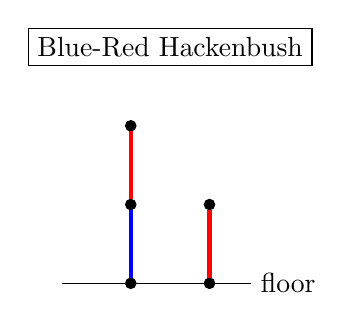
\begin{tikzpicture}
\node[draw] (title) at (1.5, 3) {Blue-Red Hackenbush};
\node (p1) at (0,0) {};
\node (p2) at (3,0) {floor};
\begin{scope} [every node/.style={scale=0.4, circle, draw, fill=black}]
	\node (p3) at (1,0) {};
	\node (p4) at (1,1) {};
	\node (p5) at (1,2) {};
	\node (p6) at (2,0) {};
	\node (p7) at (2,1) {};
	\draw (p1) -- (p2);
	\begin{scope} [ultra thick]
		\draw[blue] (p3) -- (p4);
		\draw[red] (p4) -- (p5);
		\draw[red] (p6) -- (p7);
	\end{scope}
\end{scope}
\end{tikzpicture}


In this game, a move is made by taking a single colored edge of the image and removing any edges that become disconnected from the floor. One player can only remove blue edges, and the other, red edges.

It is a common practice to assume that, unless specified otherwise, games will be played between the players \naming{Left (bLue)} and \naming{Right (Red)}.


